% questions.tex —— 2004 年·普通高等学校春季招生考试·安徽卷理科 · 题目内容片段（无答案）
% 由 tools/generate_projects.py 依来源总账自 2004/2004_数学真题_春季安徽理_试题.md 生成，勿手改（改源 MD 后重跑）


\gkpart{数学试卷}

\begin{gktip}
\textbf{来源说明}：本稿依据固定来源 PDF 转录。文件共 2 页、A3 版面，印刷页码为 149–150；PDF 元数据表明它由 XeTeX 生成，不是原始扫描件。固定文件的路径和 SHA-256 已与来源清单核对；本库将其规范绑定为 gk-2004-spring-anhui-science，仅表示此固定副本对应本卷，不代表来源身份已认证或为官方原件。上游出版物、出版者及版次尚未证实。

\textbf{答案说明}：固定 PDF 仅含试题页，没有答案页；答案与解析是本项目依据已核正题面自行推导的非官方内容，并已完成独立盲解交叉核对。官方答案字段保持为空（null）。

\textbf{图表说明}：第 20 题的三棱柱图以 TikZ 重绘为黑白矢量示意，保留可辨线段拓扑及隐藏边 AC 虚线，不按比例。详见图表清单。
\end{gktip}

\gkpart{一、选择题}

\begin{question}
\gkti{1}$\dfrac{5(4+i)^2}{i(2+i)}=$\mbox{（　　）}。

（A）$5(1-38i)$　　（B）$5(1+38i)$　　（C）$1+38i$　　（D）$1-38i$

\end{question}
\begin{question}
\gkti{2}不等式 $|2x^2-1|\leq 1$ 的解集为\mbox{（　　）}。

（A）$\{x\mid -1\leq x\leq 1\}$　　（B）$\{x\mid -2\leq x\leq 2\}$

（C）$\{x\mid 0\leq x\leq 2\}$　　（D）$\{x\mid -2\leq x\leq 0\}$

\end{question}
\begin{question}
\gkti{3}已知 $F_1,F_2$ 为椭圆 $\dfrac{x^2}{a^2}+\dfrac{y^2}{b^2}=1\ (a>b>0)$ 的焦点，$M$ 为椭圆上一点，$MF_1$ 垂直于 $x$ 轴，且 $\angle F_1MF_2=60^\circ$，则椭圆的离心率为\mbox{（　　）}。

（A）$\dfrac{1}{2}$　　（B）$\dfrac{\sqrt{2}}{2}$　　（C）$\dfrac{\sqrt{3}}{3}$　　（D）$\dfrac{\sqrt{3}}{2}$

\end{question}
\begin{question}
\gkti{4}$\displaystyle\lim_{n\to\infty}\dfrac{(n-2)^2(2+3n)^3}{(1-n)^5}=$\mbox{（　　）}。

（A）$0$　　（B）$32$　　（C）$-27$　　（D）$27$

\end{question}
\begin{question}
\gkti{5}等边三角形 $ABC$ 的边长为 $4$，$M,N$ 分别为 $AB,AC$ 的中点，沿 $MN$ 将 $\triangle AMN$ 折起，使得面 $AMN$ 与面 $MNCB$ 所处的二面角为 $30^\circ$，则四棱锥 $A-MNCB$ 的体积为\mbox{（　　）}。

（A）$\dfrac{3}{2}$　　（B）$\dfrac{\sqrt{3}}{2}$　　（C）$\sqrt{3}$　　（D）$3$

\end{question}
\begin{question}
\gkti{6}已知数列 $\{a_n\}$ 满足 $a_0=1$，$a_n=a_0+a_1+\cdots+a_{n-1}\ (n\geq 1)$，则当 $n\geq 1$ 时，$a_n=$\mbox{（　　）}。

（A）$2^n$　　（B）$\dfrac{n(n+1)}{2}$　　（C）$2^{n-1}$　　（D）$2^n-1$

\end{question}
\begin{question}
\gkti{7}若二面角 $\alpha-l-\beta$ 为 $120^\circ$，直线 $m\perp\alpha$，则 $\beta$ 所在平面内的直线与 $m$ 所成角的取值范围是\mbox{（　　）}。

（A）$(0^\circ,90^\circ]$　　（B）$[30^\circ,60^\circ]$　　（C）$[60^\circ,90^\circ]$　　（D）$[30^\circ,90^\circ]$

\end{question}
\begin{question}
\gkti{8}若 $f(\sin x)=2-\cos 2x$，则 $f(\cos x)=$\mbox{（　　）}。

（A）$2-\sin 2x$　　（B）$2+\sin 2x$　　（C）$2-\cos 2x$　　（D）$2+\cos 2x$

\end{question}
\begin{question}
\gkti{9}直角坐标 $xOy$ 平面上，平行直线 $x=n\ (n=0,1,2,\ldots,5)$ 与平行直线 $y=n\ (n=0,1,2,\ldots,5)$ 组成的图形中，矩形共有\mbox{（　　）}。

（A）$25$ 个　　（B）$36$ 个　　（C）$100$ 个　　（D）$225$ 个

\end{question}
\begin{question}
\gkti{10}已知直线 $l:x-y-1=0$，$l_1:2x-y-2=0$。若直线 $l_2$ 与 $l_1$ 关于 $l$ 对称，则 $l_2$ 的方程是\mbox{（　　）}。

（A）$x-2y+1=0$　　（B）$x-2y-1=0$　　（C）$x+y-1=0$　　（D）$x+2y-1=0$

\end{question}
\begin{question}
\gkti{11}已知向量集合 $M=\{\vec a\mid\vec a=(1,2)+\lambda(3,4),\ \lambda\in\mathbb{R}\}$，$N=\{\vec a\mid\vec a=(-2,-2)+\lambda(4,5),\ \lambda\in\mathbb{R}\}$，则 $M\cap N=$\mbox{（　　）}。

（A）$\{(1,1)\}$　　（B）$\{(1,1),(-2,-2)\}$

（C）$\{(-2,-2)\}$　　（D）$\varnothing$

\end{question}
\begin{question}
\gkti{12}函数 $y=\sin^4x+\cos^4x$ 的最小正周期为\mbox{（　　）}。

（A）$\dfrac{\pi}{4}$　　（B）$\dfrac{\pi}{2}$　　（C）$\pi$　　（D）$2\pi$

\end{question}
\gkpart{二、填空题}

\begin{question}
\gkti{13}抛物线 $y^2=6x$ 的准线方程为 $\underline{\qquad\qquad}$。

\end{question}
\begin{question}
\gkti{14}在 $5$ 名学生（$3$ 名男生，$2$ 名女生）中安排 $2$ 名学生值日，其中至少有 $1$ 名女生的概率是 $\underline{\qquad\qquad}$。

\end{question}
\begin{question}
\gkti{15}函数 $y=\sqrt{x}-x\ (x\geq 0)$ 的最大值为 $\underline{\qquad\qquad}$。

\end{question}
\begin{question}
\gkti{16}若 $\left(x+\dfrac{1}{x}-2\right)^n$ 的展开式中常数项为 $-20$，则自然数 $n=$ $\underline{\qquad\qquad}$。

\end{question}
\gkpart{三、解答题}

\begin{question}
\gkti{17}解关于 $x$ 的不等式：$\log_a^3 x<3\log_a x\ (a>0\text{ \text{且} }a\neq 1)$。

\end{question}
\begin{question}
\gkti{18}已知正项数列 $\{b_n\}$ 的前 $n$ 项和 $B_n=\dfrac{1}{4}(b_n+1)^2$，求 $\{b_n\}$ 的通项公式。

\end{question}
\begin{question}
\gkti{19}已知 $k>0$，直线 $l_1:y=kx$，$l_2:y=-kx$。

(1) 证明：到 $l_1,l_2$ 的距离的平方和为定值 $a\ (a>0)$ 的点的轨迹是圆或椭圆；

(2) 求到 $l_1,l_2$ 的距离之和为定值 $c\ (c>0)$ 的点的轨迹。

\Needspace{0.4\textheight}
\end{question}
\begin{question}
\gkti{20}已知三棱柱 $ABC-A_1B_1C_1$ 中，底面边长和侧棱长均为 $a$，侧面 $A_1ACC_1\perp$ 底面 $ABC$，$A_1B=\dfrac{\sqrt{6}}{2}a$。

(1) 求异面直线 $AC$ 与 $BC_1$ 所成角的余弦值；

(2) 求证：$A_1B\perp$ 面 $AB_1C$。
\nopagebreak[4]
\begin{center}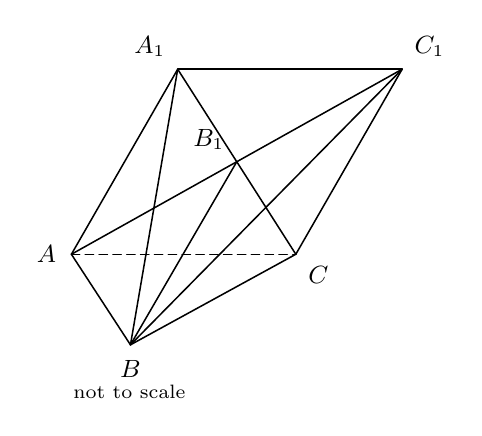
\begin{tikzpicture}[
  x=1cm,
  y=1cm,
  line cap=round,
  line join=round,
  every node/.style={font=\small},
  edge/.style={draw=black, line width=0.55pt}
]
  \coordinate (A) at (0,0);
  \coordinate (B) at (0.75,-1.15);
  \coordinate (C) at (2.85,0);
  \coordinate (A_1) at (1.35,2.35);
  \coordinate (B_1) at (2.10,1.175);
  \coordinate (C_1) at (4.20,2.35);

  % Hidden edge from the source figure.
  \draw[densely dashed, line width=0.55pt] (A) -- (C);

  % Triangular prism edges.
  \draw[edge] (A) -- (B);
  \draw[edge] (B) -- (C);
  \draw[edge] (A) -- (A_1);
  \draw[edge] (B) -- (B_1);
  \draw[edge] (C) -- (C_1);
  \draw[edge] (A_1) -- (B_1);
  \draw[edge] (B_1) -- (C_1);
  \draw[edge] (A_1) -- (C_1);

  % Additional lines appearing in the source geometry diagram.
  \draw[edge] (A_1) -- (B);
  \draw[edge] (A) -- (B_1);
  \draw[edge] (B) -- (C_1);
  \draw[edge] (B_1) -- (C);

  \node[left=2pt] at (A) {$A$};
  \node[below=2pt] at (B) {$B$};
  \node[below right=1pt] at (C) {$C$};
  \node[above left=1pt] at (A_1) {$A_1$};
  \node[above left=1pt] at (B_1) {$B_1$};
  \node[above right=1pt] at (C_1) {$C_1$};
  \node[font=\scriptsize, anchor=west] at (-0.1,-1.75) {not to scale};
\end{tikzpicture}
\end{center}
\nopagebreak[4]
\end{question}
\begin{question}
\gkti{21}已知盒中有 $10$ 个灯泡，其中 $8$ 个正品，$2$ 个次品。现需要从中取出 $2$ 个正品，每次取出 $1$ 个，取出后不放回，直到取出 $2$ 个正品为止。设 $\xi$ 为取出的次数，求 $\xi$ 的分布列及 $E\xi$。

\end{question}
\begin{question}
\gkti{22}已知抛物线 $C:y=x^2+4x+\dfrac{2}{7}$，过 $C$ 上一点 $M$，且与 $M$ 处的切线垂直的直线称为 $C$ 在点 $M$ 的法线。

(1) 若 $C$ 在点 $M$ 的法线的斜率为 $-\dfrac{1}{2}$，求点 $M$ 的坐标 $(x_0,y_0)$；

(2) 设 $P(-2,a)$ 为 $C$ 对称轴上的一点，在 $C$ 上是否存在点，使得 $C$ 在该点的法线通过点 $P$？若有，求出这些点，以及 $C$ 在这些点的法线方程；若没有，请说明理由。

\end{question}